\documentclass[12pt]{report}
\usepackage[utf8]{inputenc}
%\usepackage[14pt]{extsizes}
\usepackage{listings}
\usepackage{indentfirst}
\usepackage{geometry}
\usepackage{textcomp}
\usepackage{amssymb}
\usepackage{amsmath}
\usepackage{amsthm} 
\usepackage{caption}
\usepackage{misccorr}
\usepackage[noadjust]{cite}
\usepackage{cmap} 
\usepackage[T2A]{fontenc}
\usepackage[english, russian]{babel}
\usepackage{graphics}
\usepackage{graphicx}
\usepackage{textcomp}
\usepackage{verbatim}
\usepackage{makeidx}
\usepackage{float}
\usepackage{bm}
\usepackage{esint}
\usepackage{mathtools}
\usepackage{graphicx}
\usepackage{listings}
% Для листинга кода:
\lstset{ %
language=python,                 % выбор языка для подсветки (здесь это С)
basicstyle=\small\sffamily, % размер и начертание шрифта для подсветки кода
numbers=left,               % где поставить нумерацию строк (слева\справа)
numberstyle=\tiny,           % размер шрифта для номеров строк
stepnumber=1,                   % размер шага между двумя номерами строк
numbersep=5pt,                % как далеко отстоят номера строк от подсвечиваемого кода
showspaces=false,            % показывать или нет пробелы специальными отступами
showstringspaces=false,      % показывать или нет пробелы в строках
showtabs=false,             % показывать или нет табуляцию в строках
frame=single,              % рисовать рамку вокруг кода
tabsize=2,                 % размер табуляции по умолчанию равен 2 пробелам
captionpos=t,              % позиция заголовка вверху [t] или внизу [b] 
breaklines=true,           % автоматически переносить строки (да\нет)
breakatwhitespace=false, % переносить строки только если есть пробел
escapeinside={\#*}{*)}   % если нужно добавить комментарии в коде
}


% plot
\usepackage{pgfplots}
\usepackage{filecontents}
\usetikzlibrary{datavisualization}
\usetikzlibrary{datavisualization.formats.functions}

% Для измененных титулов глав:
\usepackage{titlesec, blindtext, color} % подключаем нужные пакеты
\definecolor{gray75}{gray}{0.75} % определяем цвет
\newcommand{\hsp}{\hspace{20pt}} % длина линии в 20pt
% titleformat определяет стиль
\titleformat{\chapter}[hang]{\Huge\bfseries}{\thechapter\hsp\textcolor{gray75}{|}\hsp}{0pt}{\Huge\bfseries}

\makeatletter
\def\@biblabel#1{#1. }
\makeatother

\usepackage{hyperref}

\newcommand{\specchapter}[1]{\chapter*{#1}\addcontentsline{toc}{chapter}{#1}}
\newcommand{\specsection}[1]{\section*{#1}\addcontentsline{toc}{section}{#1}}
\newcommand{\specsubsection}[1]{\subsection*{#1}\addcontentsline{toc}{subsection}{#1}}

% геометрия
\geometry{pdftex, left = 2cm, right = 2cm, top = 2.5cm, bottom = 2.5cm}

\titlespacing{\chapter}{0pt}{-30pt}{20pt}

\setcounter{tocdepth}{4} % фикс переноса 
\righthyphenmin = 2
\tolerance = 2048

\begin{document}
%\def\chaptername{} % убирает "Глава"
\thispagestyle{empty}
\renewcommand\bibname{Список литературы}

\vspace{\baselineskip}
\noindent \begin{minipage}{0.15\textwidth}
	
\includegraphics[width=\linewidth]{bmstu}
\end{minipage}
\noindent\begin{minipage}{0.9\textwidth}
	\centering
	\textbf{Министерство науки и высшего образования Российской Федерации}\\
	\textbf{Федеральное государственное бюджетное образовательное учреждение высшего образования}\\
	\textbf{«Московский государственный технический университет имени Н.Э.~Баумана}\\
	\textbf{(национальный исследовательский университет)»}\\
	\textbf{(МГТУ им. Н.Э.~Баумана)}
\end{minipage}

\noindent\rule{18cm}{3pt}
\newline\newline
\noindent ФАКУЛЬТЕТ $\underline{\text{«Информатика и системы управления»}}$ \newline\newline
\noindent КАФЕДРА $\underline{\text{«Программное обеспечение ЭВМ и информационные технологии»}}$\newline\newline\newline\newline\newline\newline\newline


\begin{center}
\Large\textbf{Лабораторная работа № 4}
\end{center}
\vspace{\baselineskip}
\noindent\textbf{Дисциплина} $\underline{\text{Анализ алгоритмов~~~~~~~~~~~~~~~~~~~~~~~~~~~~~~~}}$\newline\newline
\noindent\textbf{Тема} $\underline{\text{Параллельное умножение матриц~~~~~~~~~~~~~~~~~~~~~~~}}$\newline\newline
\noindent\textbf{Студент} $\underline{\text{Куликов Д. А.~~~~~~~~~~~~~~~~~~~~~~~~~~~~~~~~~~~~~~~~~~~~~}}$\newline\newline
\noindent\textbf{Группа} $\underline{\text{ИУ7-52Б~~~~~~~~~~~~~~~~~~~~~~~~~~~~~~~~~~~~~~~~~~~~~~~~~~~~~~}}$\newline\newline
\noindent\textbf{Оценка (баллы)} $\underline{\text{~~~~~~~~~~~~~~~~~~~~~~~~~~~~~~~~~~~~~~~~~~~~~~~~~~~~~}}$\newline\newline
\noindent\textbf{Преподаватель} $\underline{\text{Волкова Л. Л.~~~~~~~~~~~~~~~~~~~~~~~~~~~~~~~~~~~}}$\newline

\begin{center}
	\vfill
	Москва~---~\the\year
	~г.
\end{center}
\clearpage

\tableofcontents

\newpage
\chapter*{Введение}
\addcontentsline{toc}{chapter}{Введение}
\textbf{Матрицей} A размера $[m*n]$ называется прямоугольная таблица
чисел, функций или алгебраических выражений, содержащая m строк и n столбцов. Числа m и n определяют размер матрицы \cite{mtrbook}. 

\textbf{Умножение матриц} — одна из основных операций над матрицами.
Матрица, получаемая в результате операции умножения, называется
произведением матриц. Операция умножения двух матриц выполнима только в
том случае, если число столбцов в первом сомножителе равно числу строк во
втором; в этом случае говорят, что матрицы согласованы. В частности,
умножение всегда выполнимо, если оба сомножителя — квадратные матрицы
одного и того же порядка. Таким образом, из существования произведения AB
вовсе не следует существование произведения BA.
Алгоритмы умножения матриц активно применяются во всех областях, применяющих
линейную алгебру. Примеры использования:
\begin{itemize}
	\item компьютерная графика;
	\item физика;
	\item экономика и так далее.
\end{itemize}
\vspace{\baselineskip}

\textbf{Цель работы:} изучение возможности параллельных вычислений и использование такого подхода на практике.\vspace{\baselineskip}

В данной лабораторной работе рассматривается алгоритм умножения матриц по Винограду и его параллельная версия, представленная в двух вариантах.\vspace{\baselineskip}

\textbf{Задачи работы:}
\begin{itemize}
	\item рассмотрение алгоритма умножения матриц по Винограду;
	\item проведение сравнительного анализа алгоритма умножения матриц по Винограду и двух его параллельных версий;
	\item определение зависимости времени работы алгоритма от числа потоков исполнения и размера матриц.
\end{itemize}

\chapter{Аналитическая часть}

Если число столбцов в первой матрице совпадает с числом строк во второй, то эти две матрицы можно перемножить. У произведения будет столько же строк, сколько в первой матрице, и столько же столбцов, сколько во второй.

Пусть даны две прямоугольные матрицы А и В размерности m на n и n на k соответсвенно: 
\[ \begin{bmatrix}
	a_{1,1} & ... & a_{1,n} \\
	... & ... & ... \\
	a_{m,1} & ... & a_{m,n} \\
\end{bmatrix} \]\\

\[ \begin{bmatrix}
	b_{1,1} & ... & b_{1,k} \\
	... & ... & ... \\
	b_{n,1} & ... & b_{n,k} \\
\end{bmatrix} \]\\

В результате получим матрицу C размерности m на k:

\[ \begin{bmatrix}
	c_{1,1} & ... & c_{1,k} \\
	... & ... & ... \\
	c_{m,1} & ... & c_{m,k} \\
\end{bmatrix} \]\\


$c_{i,j} = \sum\limits_{l=1}^n a_{i,l}\cdot b_{l,j}$ называется произведением матриц A и B.

\section{Описание умножения матриц по Винограду}

Если посмотреть на результат умножения двух матриц, то видно, что каждый элемент в нем представляет собой скалярное произведение соответствующих строки и столбца исходных матриц. Можно заметить также, что такое умножение допускает предварительную обработку, позволяющую часть работы выполнить заранее.\vspace{\baselineskip}

Рассмотрим два вектора $V = (v1, v2, v3, v4)$ и $W = (w1, w2, w3, w4)$. Их скалярное произведение равно: 

$ V \cdot W=v_1 \cdot w_1 + v_2 \cdot w_2 + v_3 \cdot w_3 + v_4 \cdot w_4$ \\

Это равенство можно переписать в виде: \\
$V \cdot W=(v_1 + w_2) \cdot (v_2 + w_1) + (v_3 + w_4) \cdot (v_4 + w_3) - v_1 \cdot v_2 - v_3 \cdot v_4 - w_1 \cdot w_2 - w_3 \cdot w_4$\\

Менее очевидно, что выражение в правой части последнего равенства допускает предварительную обработку: его части можно вычислить заранее и запомнить для каждой строки первой матрицы и для каждого столбца второй. 
Это означает, что над предварительно обработанными элементами нам придется выполнять лишь первые два умножения и последующие пять сложений, а также дополнительно два сложения. 

В случае умножения матриц, строка и столбец которых преставляют собой вектора нечетного размера, схема рассчета элементов результирующей матрицы сохраняется. После чего, к каждому элементу $c_{ij}$ результирующей матрицы прибавляется число $v_{im} \cdot w_{mj}$, где $v_{im}$ - последний элемент $i$-той строки первой матрицы, $w_{mj}$ - последний элемент $j$-того столбца второй матрицы.


\section{Многопоточность}

\hspace{0.6cm} \textbf {Поток выполнения} — наименьшая единица обработки, исполнение которой может быть назначено ядром операционной системы. Реализация потоков выполнения и процессов в разных операционных системах отличается друг от друга, но в большинстве случаев поток выполнения находится внутри процесса. Несколько потоков выполнения могут существовать в рамках одного и того же процесса и совместно использовать ресурсы, такие как память, тогда как процессы не разделяют этих ресурсов. В частности, потоки выполнения разделяют инструкции процесса (его код) и его контекст (значения переменных, которые они имеют в любой момент времени).

На одном процессоре многопоточность обычно происходит путём временного мультиплексирования (как и в случае многозадачности): процессор переключается между разными потоками выполнения. Это переключение контекста обычно происходит достаточно часто, чтобы пользователь воспринимал выполнение потоков или задач как одновременное. В многопроцессорных и многоядерных системах потоки или задачи могут реально выполняться одновременно, при этом каждый процессор или ядро обрабатывает отдельный поток или задачу.

Потоки возникли в операционных системах как средство распараллеливания вычислений.

Параллельное выполнение нескольких работ в рамках одного интерактивного приложения повышает эффективность работы пользователя. Так, при работе с текстовым редактором желательно иметь возможность совмещать набор нового текста с такими продолжительными по времени операциями, как переформатирование значительной части текста, печать документа или его сохранение на локальном или удаленном диске. Еще одним примером необходимости распараллеливания является сетевой сервер баз данных. В этом случае параллелизм желателен как для обслуживания различных запросов к базе данных, так и для более быстрого выполнения отдельного запроса за счет одновременного просмотра различных записей базы. Именно для этих целей современные ОС предлагают механизм многопоточной обработки (multithreading). Понятию «поток» соответствует последовательный переход процессора от одной команды программы к другой. ОС распределяет процессорное время между потоками. Процессу ОС назначает адресное пространство и набор ресурсов, которые совместно используются всеми его потоками. 

Создание потоков требует от ОС меньших накладных расходов, чем процессов. В отличие от процессов, которые принадлежат разным, вообще говоря, конкурирующим приложениям, все потоки одного процесса всегда принадлежат одному приложению, поэтому ОС изолирует потоки в гораздо меньшей степени, нежели процессы в традиционной мультипрограммной системе. Все потоки одного процесса используют общие файлы, таймеры, устройства, одну и ту же область оперативной памяти, одно и то же адресное пространство. Это означает, что они разделяют одни и те же глобальные переменные. Поскольку каждый поток может иметь доступ к любому виртуальному адресу процесса, один поток может использовать стек другого потока. Между потоками одного процесса нет полной защиты, потому что, во-первых, это невозможно, а во-вторых, не нужно. Чтобы организовать взаимодействие и обмен данными, потокам вовсе не требуется обращаться к ОС, им достаточно использовать общую память — один поток записывает данные, а другой читает их. С другой стороны, потоки разных процессов по-прежнему хорошо защищены друг от друга.

Широко используемый подход состоит и в применении тех или иных библиотек, обеспечивающих определенный программный интерфейс (application programming interface, API) для разработки параллельных программ. В рамках такого подхода наиболее известны Windows Thread API. Однако первый способ применим только для ОС семейства Microsoft Windows, а второй вариант API является достаточно трудоемким для использования и имеет низкоуровневый характер \cite{Barkalov}.


\chapter{Конструкторская часть}
В этом разделе содержатся cхема оптимизированного алгоритма умножения матриц по Винограду и описание расспараллеливания этого алгоритма.
На вход алгоритм принимает две матрицы. На выходе выдают матрицу — результат произведения двух этих матриц.\vspace{\baselineskip}

В рамках данной лабораторной работы были предложены следующие оптимизации алгоритма умножения по Винограду:
\begin{enumerate}
	\item Замена $C[i][j] = C[i][j] + \ldots$ на $C[i][j] \text{+=} \ldots$
	\item Замена цикла по $k$ от $0$ до $N/2$ с шагом $1$ на цикл от $0$ до $N$ с шагом $2$, что убрало лишние умножения на 2
	\item Элементы $MulH$ и $MulV$ сразу высчитываются отрицательными, что убирает 1 операцию отрицания в цикле
	\item Замена $C[i][j] = \ldots$ в цикле по $k$ на буферную переменную, что убирает 2 операции индлексирования во внутреннем цикле, но добавляет С[i][j] = tmp во внешний цикл
	\item Перенос проверки четности внутрь основного цикла, что ухудшило лучший случай, но улучшило худший
	\item Вычисление условия четности и значения $N-1$, тем самым улучшая и лучший, и худший случаи
\end{enumerate}
	
\section{Схемы алгоритмов}
На Рис. 2.1 - 2.3 представлена схема оптимизированного алгоритма Винограда умножения матриц.


\newpage
\begin{figure}[h]
	\center{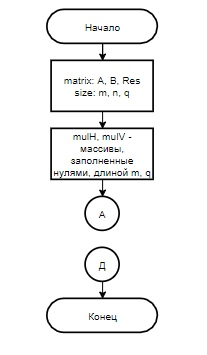
\includegraphics[scale=1]{sch1}}
	\caption{Алгоритм умножения матриц по Винограду}
	\label{figure:image}
\end{figure}

\newpage
\begin{figure}[h]
	\center{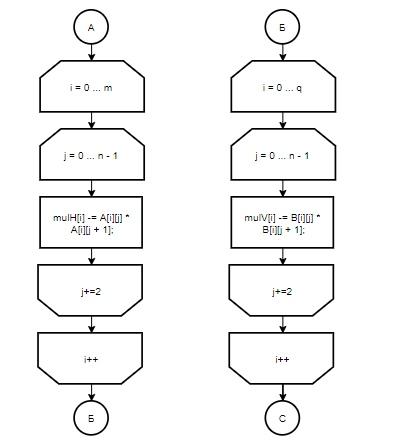
\includegraphics[scale=1]{sch2}}
	\caption{Алгоритм умножения матриц по Винограду(продолжение 1)}
	\label{figure:image}
\end{figure}

\newpage
\begin{figure}[h]
	\center{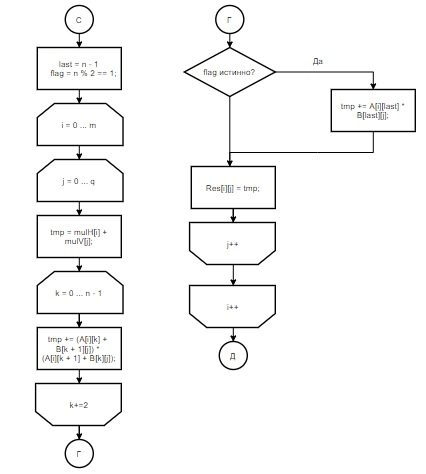
\includegraphics[scale=1]{sch3}}
	\caption{Алгоритм умножения матриц по Винограду(продолжение 2)}
	\label{figure:image}
\end{figure}


\section{Распараллеливание алгоритма Винограда}
\qquad Распараллеливание программы должно ускорять время работы. Это достигается за счет реализации в узких участках (например в циклах с большим количеством независимых вычислений).

В предложенном алгоритме данными участками  являются тройной цикл поиска результата(участок от C до Д), цикл вычисления сумм перемноженных пар строк первой матрицы и  сумм перемноженных пар столбцов второй матрицы(участок от А до C).

Данные участки программы как раз предлагается распараллелить. Задача эффективного распараллеливания алгоритма может быть решена по-разному. Ниже представлены два варианта распараллеливание алгоритма умножения матриц по Винограду.

\subsection{Распараллеливание по группам строк}
\qquad Первая версия параллельного алгоритма заключается в том, чтобы разбить строки первой матрицы на блоки с одинаковым количеством строк в каждой, за исключением, когда количество строк не кратно количеству потоков, последнего. Таким образом мы получим схему, в которой каждый поток выполняет вычисления для каждой строки из своего блока, как это показано на Рис. 2.4 (количество потоков равно 3). На нем видно, что матрица А разбита на блоки по две строки в каждом, кроме последнего, так как количество строк оказалось нечетным. Внутри каждого потока идет перемножение каждой строки, на каждый столбец матрицы B, после выполнения работы каждым из потоков на выходе получается готовая матрица

\begin{figure}[H]
	\centering
	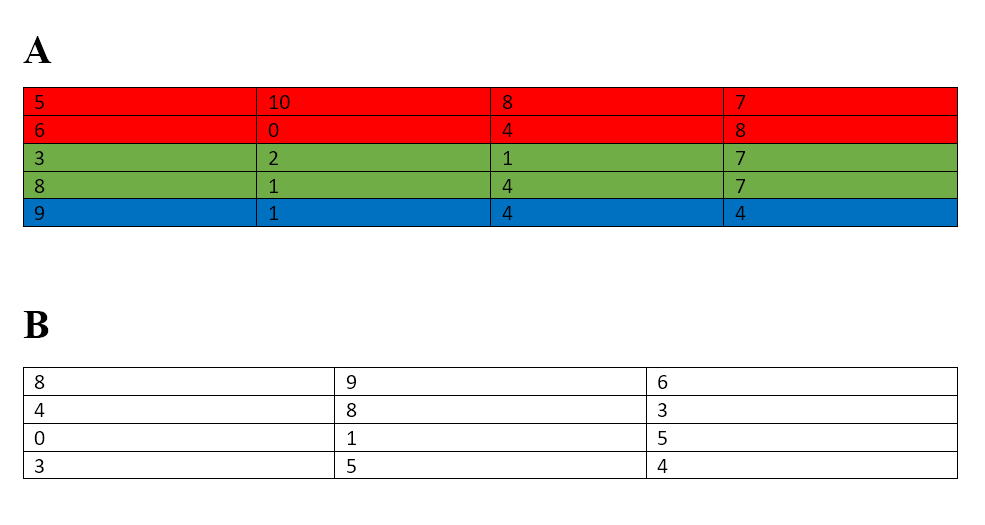
\includegraphics[scale=0.5]{ex_1}
	\caption{Версия параллельного алгоритма с разбивкой строк первой матрицы на блоки. В матрице А каждый цвет обозначает группу строк, принадлежащих отдельному потоку}
	\label{fig:mpr}
\end{figure}

При такой схеме нет проблем с обеспечением синхнонизации, так как каждый блок независим от другого, и вычисления в одном ни как не влияют на вычисления в другом.

\subsection{Распараллеливание по строке}
\quad Данный подход заключается в том, чтобы каждый поток занимался обработкой лишь одной строки. В отличие от предыдущего варинта, он будет сложнее в реализации, в силу необходимости обеспечения синхронизации между потоками.
На вход подается определенное количество потоков, которое необязательно будет равно количеству строк в таблице, следовательно, возникает следующая проблема: как поток, после обработки строки, будет понимать какую следующую строчку ему обрабатывать? Для решения этого вопроса необходимо создать очередь, в которой будут лежать индексы тех строк, которые еще не были обработаны. Каждый поток будет обращаться к этой очереди и "брать себе задачу", то есть получать индекс строки, которую нужно обработать, после чего повторит эти действия. Разделение первой матрицы 2 потоками представлено на Рис 2.5. Несмотря на то, что на нем каждая строка закрашена одним из двух цветов(так как имеется в данном примере только 2 потока), эти строки не обрабатываются сразу. Сначала 1 и 2 поток захватят индекс 1 и 2 строки соответственно, произведут над ними вычисления, а затем перейдут к строке 3 и 4 и т.д.

\begin{figure}[!htbp]
	\centering
	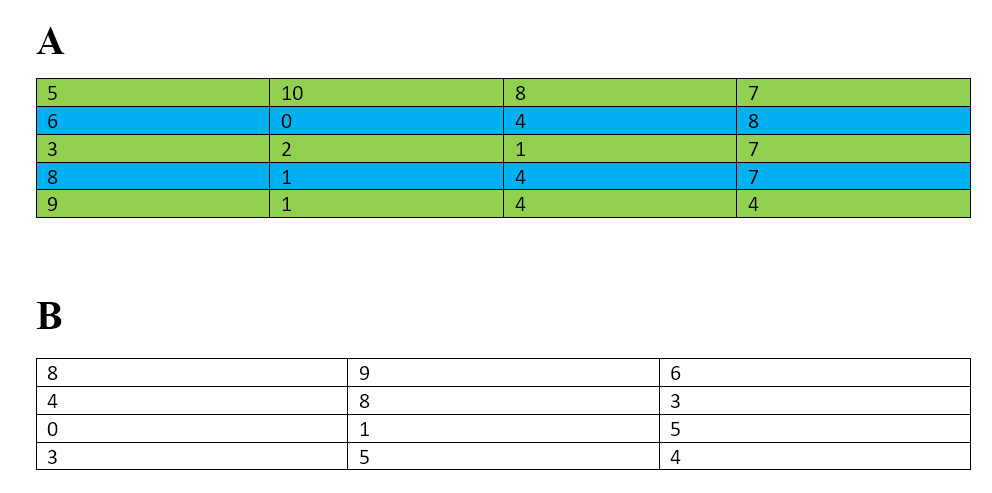
\includegraphics[scale=0.5]{ex_2}
	\caption{Версия параллельного алгоритма с построчной обработкой матрицы каждым потоком. В матрице А каждый цвет обозначает строку, которая будет обработана конкретным потоком}
	\label{fig:mpr}
\end{figure}

\qquad Проблема заключается в захвате индекса следующей строки из очереди. Потоки работают внутри одного процесса, а следовательно разделяют его общую память. Если один поток получит значение из очереди, то другой может просто "не увидеть" этого и обработать эту же строку, что приведет к неверному ответу. Для того чтобы синхронизировать потоки, необходимо воспользоваться мьютексом. Мьютекс - примитив синхронизации, который позволяет захватить владение каким-либо объектом определенным потоком, в таком случае другие потоки не смогут каким-либо образом повлиять на данный объект, пока данный поток не вернет его в общее пользование.\cite{voevodin}

\chapter{Технологическая часть}
В данном разделе будут рассмотрены требования к программному обеспечению, средства реализации, представлен листинг кода и описание тестирования.
\section{Требования к программному обеспечению}
\textbf{Требования к вводу:} на вход подаются две матрицы, размеры которых m x n и n x q соответственно. 

\textbf{Требования к программе:}
\begin{enumerate}
	\item на выходе
	необходимо получить матрицу, которая является результатом умножения двух матриц;
	\item требуется замерить время работы
	каждого из алгоритмов. 
\end{enumerate}
\section{Средства реализации}
В качестве языка программирования был выбран С++ т.к. я знаком с данным языком, у него есть уникальный баланс между возможностями объектно-ориентированного программирования и производительностью. Он одновременно позволяет писать высокоуровневый абстрактный код, который при этом работает со скоростью близкой к машинному коду.

Среда разработки — Visual Studio, которая предоставляет умную проверку кода, быстрое выявление ошибок и оперативное исправление, вкупе с автоматическим рефакторингом кода, и богатыми возможностями в навигации.  

Время работы алгоритмов было замерено с помощью функции steady\_clock() из библиотеки chrono \cite{chrono}. 

Для тестирования использовался компьютер на базе процессора Intel(R) Core(TM) i5-4200U, 2 ядра, 4 логических процессоров. 

Многопоточное программирование было
реализовано с помощью библиотеки thread \cite{thread}.

\newpage
\section{Листинг кода}

\hspace{0.2cm}В Листинге 3.1 показана реализация оптимизированного алгоритма умножения матриц по Винограду.

\begin{lstlisting}[label=some-code,caption=Оптимизированный алгоритм умножения матриц по Винограду]
int vinogradOPT(const vector<vector<int>>& A, const vector<vector<int>>& B,
const int m, const int n, const int q, vector<vector<int>>& C)
{
	vector<int> mulH(m, 0);
	for (int i = 0; i < m; i++)
	{
		for (int j = 0; j < n - 1; j += 2)
		{
			mulH[i] -= A[i][j] * A[i][j + 1];
		}
	}
	
	vector<int> mulV(q, 0);
	for (int i = 0; i < q; i++)
	{
		for (int j = 0; j < n - 1; j += 2)
		{
			mulV[i] -= B[j][i] * B[j + 1][i];
		}
	}
	int last = n - 1;
	bool flag = n % 2 == 1;
	C = vector<vector<int>>(m, vector<int>(q, 0));
	for (int i = 0; i < m; i++)
	{
		for (int j = 0; j < q; j++)
		{
			int tmp = mulH[i] + mulV[j];
			for (int k = 0; k < n - 1; k += 2)
			{
				tmp += (A[i][k] + B[k + 1][j]) * (A[i][k + 1] + B[k][j]);
			}
			if (flag)
			{
				tmp += A[i][last] * B[last][j];
			}
			C[i][j] = tmp;
		}
	}
	return OK;
}
\end{lstlisting}

В Листингах 3.2 - 3.5 показана реализация распараллеленного по группам строк оптимизированного алгоритма умножения матриц по Винограду.
\begin{lstlisting}[label=some-code,caption=Многопоточного оптимизированный алгоритм умножения матриц по Винограду]
int threadedVinogradOPT1(const vector<vector<int>>& A, const vector<vector<int>>& B,
const int m, const int n, const int q, vector<vector<int>>& C,
const int& nThreads)
{
	vector<thread> threads;
	vector<int> mulH(m, 0);
	double start = 0;
	double del = m / static_cast<double>(nThreads);
	for (int i = 0; i < nThreads; i++)
	{
		threads.push_back(thread(computeMulH, ref(mulH), A, round(start),
		round(start + del)));
		start += del;
	}
	for (auto& thread : threads)
	{
		thread.join();
	}
	start = 0;
	del = q / static_cast<double>(nThreads);
	vector<int> mulV(q, 0);
	for (int i = 0; i < nThreads; i++)
	{
		threads[i] = thread(computeMulV, ref(mulV), B, round(start),
		round(start + del));
		start += del;
	}
	for (auto& thread : threads)
	{
		thread.join();
	}
	
	C = vector<vector<int>>(m, vector<int>(q, 0));
	start = 0;
	del = m / static_cast<double>(nThreads);
	for (int i = 0; i < nThreads; i++)
	{
		threads[i] = thread(computeResult, ref(C), A, B, 
		mulH, mulV, round(start), round(start + del));
		start += del;
	}
	for (auto& thread : threads)
	{
		thread.join();
	}
	return OK;
}
\end{lstlisting}

\begin{lstlisting}[label=some-code,caption=Функция вычисления сумм строк первой матрицы]
void computeMulH(vector<int>& mulH, vector<vector<int>> A, int startRow, int endRow)
{
	int n = A[0].size();
	for (int i = startRow; i < endRow; i++)
	{
		for (int j = 0; j < n - 1; j += 2)
		{
			mulH[i] -= A[i][j] * A[i][j + 1];
		}
	}
}
\end{lstlisting}

\begin{lstlisting}[label=some-code,caption=Функция вычисления сумм столбцов второй матрицы]
void computeMulV(vector<int>& mulV, vector<vector<int>> B, int startCol, int endCol)
{
	int n = B.size();
	for (int i = startCol; i < endCol; i++)
	{
		for (int j = 0; j < n - 1; j += 2)
		{
			mulV[i] -= B[j][i] * B[j + 1][i];
		}
	}
}
\end{lstlisting}

\newpage
\begin{lstlisting}[label=some-code,caption=Функция вычисления результирующей матрицы]
void computeResult1(vector<vector<int>>& C, vector<vector<int>> A,
vector<vector<int>> B, vector<int> mulH,
vector<int> mulV, int startRow, int endRow)
{
	int n = B.size();
	int q = B[0].size();
	int last = n - 1;
	bool flag = n % 2 == 1;
	for (int i = startRow; i < endRow; i++)
	{
		for (int j = 0; j < q; j++)
		{
			int tmp = mulH[i] + mulV[j];
			for (int k = 0; k < n - 1; k += 2)
			{
				tmp += (A[i][k] + B[k + 1][j]) * (A[i][k + 1] + B[k][j]);
			}
			if (flag)
			{
				tmp += A[i][last] * B[last][j];
			}
			C[i][j] = tmp;
		}
	}
}
\end{lstlisting}

\newpage
В Листингах 3.6 - 3.7 показана реализация распараллеленного по строке оптимизированного алгоритма умножения матриц по Винограду.
\begin{lstlisting}[label=some-code,caption=Функция вычисления результирующей матрицы]
int threadedVinogradOPT2(const vector<vector<int>>& A, const vector<vector<int>>& B,
const int m, const int n, const int q, vector<vector<int>>& C,
const int& nThreads)
{
	vector<thread> threads;
	vector<int> mulH(m, 0);
	double start = 0;
	double del = m / static_cast<double>(nThreads);
	for (int i = 0; i < nThreads; i++)
	{
		threads.push_back(thread(computeMulH, ref(mulH), A, round(start),
		round(start + del)));
		start += del;
	}
	for (auto& thread : threads)
	{
		thread.join();
	}
	start = 0;
	del = q / static_cast<double>(nThreads);
	vector<int> mulV(q, 0);
	for (int i = 0; i < nThreads; i++)
	{
		threads[i] = thread(computeMulV, ref(mulV), B, round(start),
		round(start + del));
		start += del;
	}
	for (auto& thread : threads)
	{
		thread.join();
	}
	
	C = vector<vector<int>>(m, vector<int>(q, 0));
	queue<int> que;
	
	for (int i = 0; i < m; i++)
	que.push(i);
	for (int i = 0; i < nThreads; i++)
	{
		threads[i] = thread(computeResult1, ref(C), A, B,
		mulH, mulV, ref(que));
	}
	for (auto& thread : threads)
	{
		thread.join();
	}
	return OK;
}
\end{lstlisting}

\newpage
\begin{lstlisting}[label=some-code,caption=Функция вычисления результирующей матрицы]
void computeResult1(vector<vector<int>>& C, vector<vector<int>> A,
vector<vector<int>> B, vector<int> mulH,
vector<int> mulV, queue<int> &que)
{
	int n = B.size();
	int q = B[0].size();
	int last = n - 1;
	bool flag = n % 2 == 1;
	mutex m;
	while (true) 
	{
		m.lock();
		if (que.empty()) 
		{
			m.unlock();
			break;
		}
		int i = que.front();
		que.pop();
		m.unlock();
		for (int j = 0; j < q; j++)
		{
			int tmp = mulH[i] + mulV[j];
			for (int k = 0; k < n - 1; k += 2)
			{
				tmp += (A[i][k] + B[k + 1][j]) * (A[i][k + 1] + B[k][j]);
			}
			if (flag)
			{
				tmp += A[i][last] * B[last][j];
			}
			C[i][j] = tmp;
		}
	} 
}
\end{lstlisting}

\newpage
\section{Тестирование}
Реализовано функциональное тестирование отдельным файлом test.сpp. Полученные результаты функций сравниваются с контрольными значениями. \vspace{\baselineskip}

Тестирование происходит по следующим данным:
\begin{enumerate}
	\item проверка работы умножения на единичную матрицу;
	\item проверка работы умножения матрицы 3x2 на матрицу 2x4;
	\item проверка работы умножения матриц 10x10;
	\item проверка работы умножения матриц 11x11;
\end{enumerate}

Программа успешно прошла все тестовые случаи, см. Рис. 3.1. 

\begin{figure}[h]
	\center{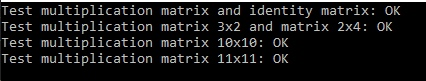
\includegraphics[scale=1]{testing}}
	\caption{Тестирование программы}
	\label{figure:image}
\end{figure}

\chapter{Экспериментальная часть}

В данном разделе приведены примеры работы программы и сравнительный анализ алгоритмов на основе экспериментальных данных. 

\section{Примеры работы} 

На Рис. 4.1 - 4.2 приведены примеры работы программы.

\begin{figure}[h]
	\center{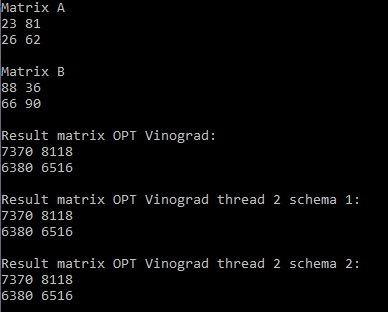
\includegraphics[scale=1]{d2}}
	\caption{Пример работы программы 2 потока}
	\label{figure:image}
\end{figure}

\begin{figure}[h]
	\center{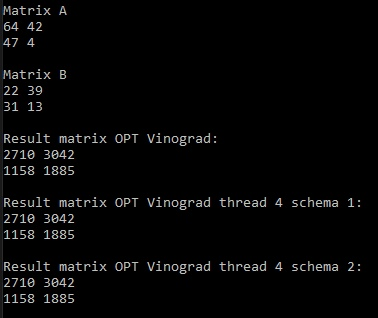
\includegraphics[scale=1]{d1}}
	\caption{Пример работы программы 4 потока}
	\label{figure:image}
\end{figure}

\newpage
\section{Постановка эксперимента по замеру времени}

Для произведения замеров времени выполнения реализации алгоритмов будет использована формула: \begin{equation}\label{eq:fourierrow}
	t = \frac{T}{N}
\end{equation}
где t — среднее время выполнения алгоритма, N — количество замеров, T — время выполнения N замеров.  
Неоднократное измерение времени необходимо для получения более точного результа.  
 
 \qquad Все эксперименты производятся на квадратных матрицах размером от 100 x 100 до 1000 x 1000 c шагом 100. Время измеряется в микросекундах.
 
 На рисунке 4.1 изображены графики зависимости времени выполнения программы от размера входных квадратных матриц и количество потоков для 1 параллельной версии классического алгоритма :  
 
 \begin{tikzpicture}
 	\begin{axis}[
 		axis lines = left,
 		xlabel = {Размер матрицы},
 		ylabel = {Время (мкс)},
 		legend pos=north west,
 		ymajorgrids=true
 		]
 		\addplot[color=red, mark=square] table[x index=0, y index= 1] {row_blocks1.txt}; 
 		\addplot[color=green, mark=square] table[x index=0, y index= 1] {row_blocks2.txt}; 
 		\addplot[color=blue, mark=square] table[x index=0, y index= 1] {row_blocks4.txt}; 
 		\addplot[color=orange, mark=triangle] table[x index=0, y index= 1] {row_blocks8.txt}; 
 		\addplot[color=brown, mark=circle] table[x index=0, y index= 1] {row_blocks16.txt}; 
 		
 		\addlegendentry{1 поток}
 		\addlegendentry{2 потока}
 		\addlegendentry{4 потока}
 		\addlegendentry{8 потоков}
 		\addlegendentry{16 потоков}
 		
 	\end{axis}
 \end{tikzpicture}
 \begin{center}
 	Pис. 4.1: Сравнение времени работы первой параллельной версии алгоритма при различном количестве потоков
 \end{center}
 
 
 Как видно из рисунка, начиная с 4 потоков увеличение числа потоков не дало сильного прироста в скорости, это связано с тем, что число потоков, которые  работают параллельно равно числу логических процессоров, которых на экспериментальном процессоре, как было сказано в Технологической части 4.
 
 
 На рисунке 4.2 изображены графики зависимости времени выполнения программы от размера входных квадратных матриц и количество потоков для 2 параллельной версии классического алгоритма : 
 
 \begin{tikzpicture}
 	\begin{axis}[
 		axis lines = left,
 		xlabel = {Размер матрицы},
 		ylabel = {Время (мкс)},
 		legend pos=north west,
 		ymajorgrids=true
 		]
 		\addplot[color=red, mark=square] table[x index=0, y index= 1] {row_strings1.txt}; 
 		\addplot[color=green, mark=square] table[x index=0, y index= 1] {row_strings2.txt}; 
 		\addplot[color=blue, mark=square] table[x index=0, y index= 1] {row_strings4.txt}; 
 		\addplot[color=orange, mark=triangle] table[x index=0, y index= 1] {row_strings8.txt}; 
 		\addplot[color=brown, mark=circle] table[x index=0, y index= 1] {row_strings16.txt}; 
 		
 		\addlegendentry{1 поток}
 		\addlegendentry{2 потока}
 		\addlegendentry{4 потока}
 		\addlegendentry{8 потоков}
 		\addlegendentry{16 потоков}
 		
 	\end{axis}
 \end{tikzpicture}
 \begin{center}
 	Pис. 4.2: Сравнение времени работы второй параллельной версии алгоритма при различном количестве потоков
 \end{center}
 
 Видно, что ситуация повторилась как и в случае с 1 версией.
 
 Так как максимальную производительность в обоих случаях удается достичь при 4 потоках, то классический метод стоит сравнивать с параллельными вресиями именно при нем.
 
 На рисунке 4.3 видно, что обе параллельные версии работают приблизительно одинаково и существенно выигрывают по времени в сравнении с классическим алгоритмом, особенно при увеличении размерности матрицы.
 
 \begin{tikzpicture}
 	\begin{axis}[
 		axis lines = left,
 		xlabel = {Размер матрицы},
 		ylabel = {Время (мкс)},
 		legend pos=north west,
 		ymajorgrids=true
 		]
 		\addplot[color=red, mark=square] table[x index=0, y index= 1] {simple.txt}; 
 		\addplot[color=green, mark=square] table[x index=0, y index= 1] {row_strings4.txt}; 
 		\addplot[color=blue, mark=square] table[x index=0, y index= 1] {row_blocks4.txt};
 		
 		\addlegendentry{Классический алгоритм}
 		\addlegendentry{1 параллельный 4 потока}
 		\addlegendentry{2 параллельный 4 потока}
 		
 	\end{axis}
 \end{tikzpicture}
 \begin{center}
 	Pис. 4.3: Сравнение времени работы классического алгоритма и двух его параллельных версий при количестве потоков равных 4
 \end{center}
 
 
 \section*{Вывод}
 \qquad По результатам исследования получилось, что обе параллельные версии алгоритма работают приблизительно за равное время, но каждая из них быстрее классического алгоритма, причем с увеличением размерности матрицы выигрыш становится все более ощутимым. Также установлено, что увеличение количества потоков имеет смысл, пока не будет достигнуто число, равное количеству логических процессоров в системе, причем самой быстрой версией параллельного алгоритма( любой из его версий) является та, гда число потоков равно числу логических процессоров.

\newpage
\chapter*{Заключение}
\addcontentsline{toc}{section}{Заключение}
\hspace{0.6cm}В ходе лабораторной работы были изучены возможности параллельных вычислений и использованы на практике. Был реализован алгоритм умножения матриц по Винограду с помощью параллельных вычислений.
Было произведено сравнение работы обычного алгоритма Винограда и параллельной реализации при увеличении количества потоков. Экспериментально было установлено, что параллельные версии быстрее классического алгоритма, причем чем больше размерность матрицы, тем больше выигрыш. Было установлено, что увеличение потоков имеет смысл, пока не будет достигнуто число логических процессоров в системе, причем максимальная скорость работы достигается именно при нем.
 
 Цель работы достигнута. Получены практические навыки использования параллельных вычислений, а также проведена исследовательская работа по временной эффективности такого подхода.     


\begin{thebibliography}{2}
	\addcontentsline{toc}{chapter}{Список литературы}
	\bibitem{mtrbook} Курош А. Г. Курс высшей алгебры. — 9-е изд. — М.: Наука, 1968. — 432 с
	\bibitem{Barkalov}
	Константин Баркалов, Владимир Воеводин, Виктор Гергель. Intel Parallel Programming [электронный ресурс]. Режим доступа: https://www.intuit.ru/studies/courses/4447/983/lecture/14925, свободный (Дата обращения: 15.10.20)
	\bibitem{voevodin}Воеводин В. В., Воеводин Вл. В. Параллельные вычисления. — СПб: БХВ-Петербург, 2002. — 608 с.
	\bibitem{chrono} Официальный сайт Microsoft, документация [электронный ресурс]. Режим доступа: https://docs.microsoft.com/ru-ru/cpp/standard-library/chrono?view=vs-2017, свободный (Дата обращения: 15.10.20)
	\bibitem{thread} Официальный сайт Microsoft, документация [электронный ресурс]. Режим доступа: https://docs.microsoft.com/ru-ru/cpp/standard-library/thread-class?view=vs-2019, свободный (Дата обращения: 15.10.20)
	
\end{thebibliography}
\end{document}